\section{单纯理论的公理}
\sourcepage{174--175}
验证公理之前，必须更仔细地处理几个问题。公理要求在容许空间类上定义同调群。严格地说，我们只对单纯复形定义了群，并未对空间定义。一个多面体可以由许多不同复形实现，它们的同调群自然同构，却仍是不同的群。同样，连续映射 $h:X\to Y$ 在选择 $X=|K|,Y=|L|$ 后诱导 $H_p(K)\to H_p(L)$，换成其他复形又得到另一同态，却都记为 $h_*$。此前已经指出这种记号歧义。

解决方法是再作一层抽象：将所有底空间为 $X$ 的复形的同调群自然地等同，所得群称为空间的同调群。更一般地，可对任何同胚于多面体的空间这样做，细节如下。

\entry{定义}{3.6.1}空间偶 $(X,A)$ 的一个\textbf{三角剖分}是复形 $K$、子复形 $K_0$ 及同胚 $h:(|K|,|K_0|)\to(X,A)$。若存在，称其为\textbf{可三角剖分偶}。$A$ 为空时，与定义 2.9.7 一致，只称 $X$ 可三角剖分。

设 $(X,A)$ 可三角剖分，考虑其全部三角剖分 $h_\alpha:(|K_\alpha|,|C_\alpha|)\to(X,A)$。这里存在类似“所有集合的集合”的集合论问题。为避免它，要求各 $K_\alpha$ 位于固定空间 $E^J$。只要 $J$ 足够大，每个复形都有同构副本位于其中；例如可取 $J$ 的基数等于 $X$ 的基数。限定在固定空间之后，就能用足够大的指标集编号。

固定 $p$，用 $H_p(K_\alpha,C_\alpha)\times\{\alpha\}$ 使各群作为集合不交。在不交并
\[
\coprod_\alpha H_p(K_\alpha,C_\alpha)\times\{\alpha\}\tag{$*$}
\]
上定义等价关系：$(x,\alpha)$ 与 $(y,\beta)$ 等价，当且仅当 $(h_\beta^{-1}h_\alpha)_*(x)=y$。定义 $H_p(X,A)$ 为这些等价类的集合。

每个等价类在每个带标签群中恰有一个元素，所以将元素映到其等价类的映射为双射。要求它成为群同构，以此给 $H_p(X,A)$ 群结构。因为各过渡映射 $(h_\beta^{-1}h_\alpha)_*$ 都为同构，此结构无歧义。

\sourcepage{176}
连续映射 $h:(X,A)\to(Y,B)$ 也诱导同态。任选两偶的剖分 $h_\alpha:(|K_\alpha|,|C_\alpha|)\to(X,A)$ 和 $k_\beta:(|L_\beta|,|D_\beta|)\to(Y,B)$，形成 $h'=k_\beta^{-1}hh_\alpha$。其诱导同态 $h'_*:H_p(K_\alpha,C_\alpha)\to H_p(L_\beta,D_\beta)$ 通过等价类给出良定义的 $h_*:H_p(X,A)\to H_p(Y,B)$。

同样，复形上的边界同态诱导 $\partial_*:H_p(X,A)\to H_{p-1}(A)$。同调理论所需的各部分已经齐备。

可三角剖分偶构成容许类：所要求的 $(X,X),(X,\varnothing),(A,A),(A,\varnothing)$ 显然可剖分，单点空间可剖分，乘积偶则由引理 2.7.3 得到。

\entry{定理}{3.6.2}可三角剖分偶上的单纯同调满足 Eilenberg--Steenrod 公理。

\noindent\textbf{证明：}公理 1--5、7 是已熟悉的复形同调性质，立即推广到空间偶。只需进一步思考紧支撑和切除公理。

先证紧支撑。设 $\alpha\in H_p(K,K_0)$，取代表链 $c$，其边界由 $K_0$ 承载。$c$ 由某个有限子复形 $L$ 承载，因此可视为相对偶 $(L,L_0)$ 的闭链，其中 $L_0=K_0\cap L$。其同调类 $\beta$ 在包含诱导映射下映为 $\alpha$，而这个偶紧致，公理得证。

切除公理的微妙之处是：两个偶即使都可三角剖分，剖分之间也可能全无关系。若两个剖分相容，结论直接由定理 1.10.6 得到。具体地，设 $U\subset A\subset X$，且剖分 $h:(|K|,|K_0|)\to(X,A)$ 还诱导 $X\setminus U$ 的剖分，即 $X\setminus U=h(|L|)$，$L$ 为子复形。令 $L_0=L\cap K_0$，则 $A\setminus U=h(|L_0|)$。此时 $U$ 开，$A$ 闭，定理 1.10.6 给出所需同构。

\sourcepage{177--178}
一般地，设 $U\subset\Int A$，分别取两偶的剖分
\[
h:(|K|,|K_0|)\to(X,A),\qquad
k:(|M|,|M_0|)\to(X\setminus U,A\setminus U).
\]
令 $X_1=\overline{X\setminus A}$，$A_1=X_1\cap A$。断言两个剖分都诱导 $(X_1,A_1)$ 的剖分，见图 3.6.1。
\begin{center}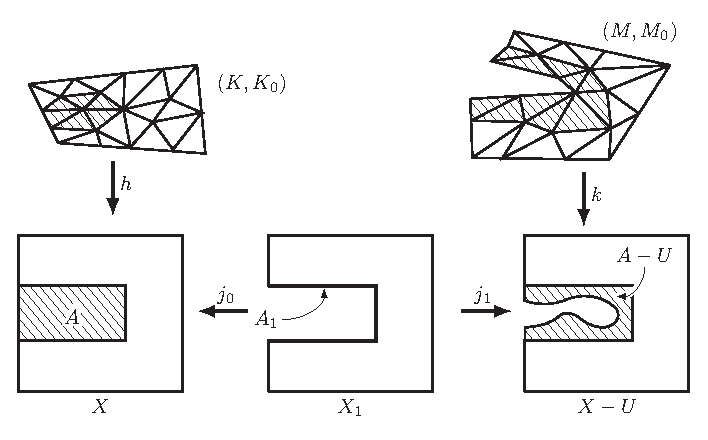
\includegraphics[width=122mm]{figures/3-6-1.pdf}\\图 3.6.1\end{center}
事实上，$|K|\setminus|K_0|$ 是所有 $\sigma\notin K_0$ 的开单形 $\Int\sigma$ 的并，其闭包 $C$ 是由这些单形及其面组成的子复形的多胞体。$h(C)=X_1$，所以 $h$ 剖分 $X_1$，也剖分交集 $A_1$。同样，$|M|\setminus|M_0|$ 的闭包是子复形的多胞体，其像为 $(X\setminus U)\setminus(A\setminus U)=X\setminus A$ 的闭包，即 $X_1$，并同时剖分 $A_1$。这里使用了 $U\subset\Int A$，保证该闭包不接触 $U$。

由已证特殊情形，包含 $j_0:(X_1,A_1)\to(X,A)$ 与 $j_1:(X_1,A_1)\to(X\setminus U,A\setminus U)$ 均诱导同构。因 $j_0=jj_1$，中间包含 $j$ 也诱导同构，完成证明。\hfill$\square$

注意，并未使用完整的切除公理假设：不要求 $\overline U\subset\Int A$，也不要求 $U$ 开。因此有更强结论。

\entry{定理}{3.6.3（单纯理论的切除）}若 $U\subset\Int A\subset X$，且 $(X,A)$ 与 $(X\setminus U,A\setminus U)$ 均可三角剖分，则包含诱导同构 $H_p(X\setminus U,A\setminus U)\cong H_p(X,A)$。

紧支撑公理大致说，每个同调类都有紧支撑。同调类之间的每个同调关系也有紧支撑，精确表述如下。先对单纯理论直接证明，也可由公理导出，见习题。

\entry{定理}{3.6.4}设 $i:(X_0,A_0)\to(X,A)$ 为可三角剖分偶的包含，$(X_0,A_0)$ 紧致。若 $\alpha\in H_p(X_0,A_0)$ 且 $i_*(\alpha)=0$，则存在紧致可三角剖分偶 $(X_1,A_1)$ 及包含 $(X_0,A_0)\xrightarrow{j}(X_1,A_1)\xrightarrow{k}(X,A)$，使 $j_*(\alpha)=0$。

\noindent\textbf{证明：}不妨设 $(X,A)=(|K|,|C|)$。因为 $X_0$ 紧致，包含在某个有限子复形 $K_0$ 的多胞体中；$A_0$ 位于 $|C_0|$，其中 $C_0=C\cap K_0$。故可归结为有限子复形偶的包含 $(K_0,C_0)\to(K,C)$。

取代表 $\alpha$ 的链 $c_p$。其像为零，所以存在 $d_{p+1}$，使 $c_p-\partial d_{p+1}$ 由 $C$ 承载。选 $C$ 的有限子复形承载此差，连同 $C_0$ 取并为 $C_1$。再选 $K$ 的有限子复形承载 $d_{p+1}$，连同 $K_0,C_1$ 取并为 $K_1$。则 $(K_0,C_0)\to(K_1,C_1)$ 已把 $\alpha$ 映到零。\hfill$\square$

\sourcepage{179--180}
\entry{定理}{3.6.5}给定有限生成阿贝尔群序列 $G_0,G_1,\ldots$，其中 $G_0$ 自由且非零，则存在复形 $K$，使每个 $H_i(K)\cong G_i$。

证明留作习题。

\subsection*{习题}
\begin{enumerate}
\item 证明定理 3.6.5。［提示：第 3.4 节习题 5。］
\item 设容许类为所有可三角剖分偶，或所有拓扑空间偶。直接从公理证明定理 3.6.4，其中将“可三角剖分”均换成“容许”。

［提示：可三角剖分情形可以假设 $(X,A)$ 的剖分也剖分 $X_0$。考察图
\begin{center}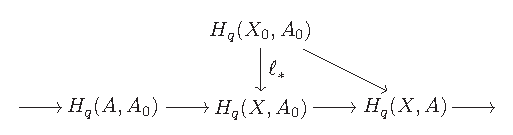
\includegraphics[width=99mm]{figures/3-6-ex-a.pdf}\end{center}
找出紧致 $A_1$，使 $\ell_*(\alpha)$ 位于 $H_q(A_1,A_0)\to H_q(X,A_0)$ 的像中。于是包含 $(X_0,A_0)\to(X,A_1)$ 将 $\alpha$ 映为零。再考察图
\begin{center}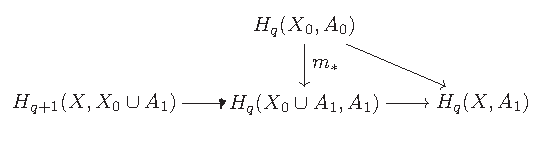
\includegraphics[width=103mm]{figures/3-6-ex-b.pdf}\end{center}
找出紧致 $X_1$，使 $m_*(\alpha)$ 位于 $\partial_*:H_{q+1}(X_1,X_0\cup A_1)\to H_q(X_0\cup A_1,A_1)$ 的像中，然后完成证明。］
\item 给出三个不同的可三角剖分偶的例子。
\end{enumerate}
